%%%%%%%%%%%%%%%%%%%%%%%%%%%%%%%%%%%%%%%%%%%%%%%%%%%%%%%%%%%%%%%%%%%%%%%%%%%%%%%%
%2345678901234567890123456789012345678901234567890123456789012345678901234567890
%        1         2         3         4         5         6         7         8
% THESIS CHAPTER

% short summary of the chapter
\section*{Summary}
On this section it will be demonstrated the results of different textures being applied to a SAR image and it will be analyzed which textures, if any, might help improve classification algorithms for forest areas and deforested areas. On this section it will be presented textures results of images of the coherence between 2 SAR images, and radar brightness ($\beta^0$)

\section{The GLCM Textures} 
\label{sec:gv1}

\subsection{The Displacement Vector}
\label{subsec:displacement_vector}
The first step to compute the textures of a image using the GLCM method is to choose the displacement vector $d=(d_1, d_2)$ that will be used to compute the grey level co-occurrence matrix. As said in the previous chapter, one way to choose this value is to use a statistical test proposed by \cite{Zucker} to find the value of $d$ that gives more texture information.
The process to compute to find the best $d$ consists of computing the grey level co-occurrence matrix for different displacement vectors and extracting the chi-squared statistical value for that occurrence matrix. The chi-square value is given by:
\begin{equation}
    \label{eq:test}
    \chi^2(d) = (\sum_i\sum_j \frac{N_d^2(i,j)}{\sum_jN_d(i,j)\sum_iN_i(i,j)} -1)
\end{equation}

It is expected that the closer the distance between the pixels the better, since pixels that are more close together in the image have bigger correlation between them. This statistical test will be run on coherence images over Amazon forest and $\beta^0$ images over Amazon forest to confirm that pixels that are closer have greater correlation between them.  
% \begin{figure}
%   \centering
%   \subfloat[]{
%     \label{fig:cap4_beta0}
%     \input{Chapter4/coSSC_master_beta0.png}
%   }
%   \subfloat[]{
%     \label{fig:cap5_gammavol}
%     \input{Chapter4/coSSC_master_gamma_vol.png}
%   }
% \end{figure}

\begin{figure}[H]
  \centering
    \begin{subfigure}[b]{0.4\linewidth}
      \includegraphics[width=0.8\linewidth]{Chapter4/coSSC_master_beta0.png}
      \caption{$\beta^0$ Image of Amazon area}
    \end{subfigure}
    \begin{subfigure}[b]{0.4\linewidth}
      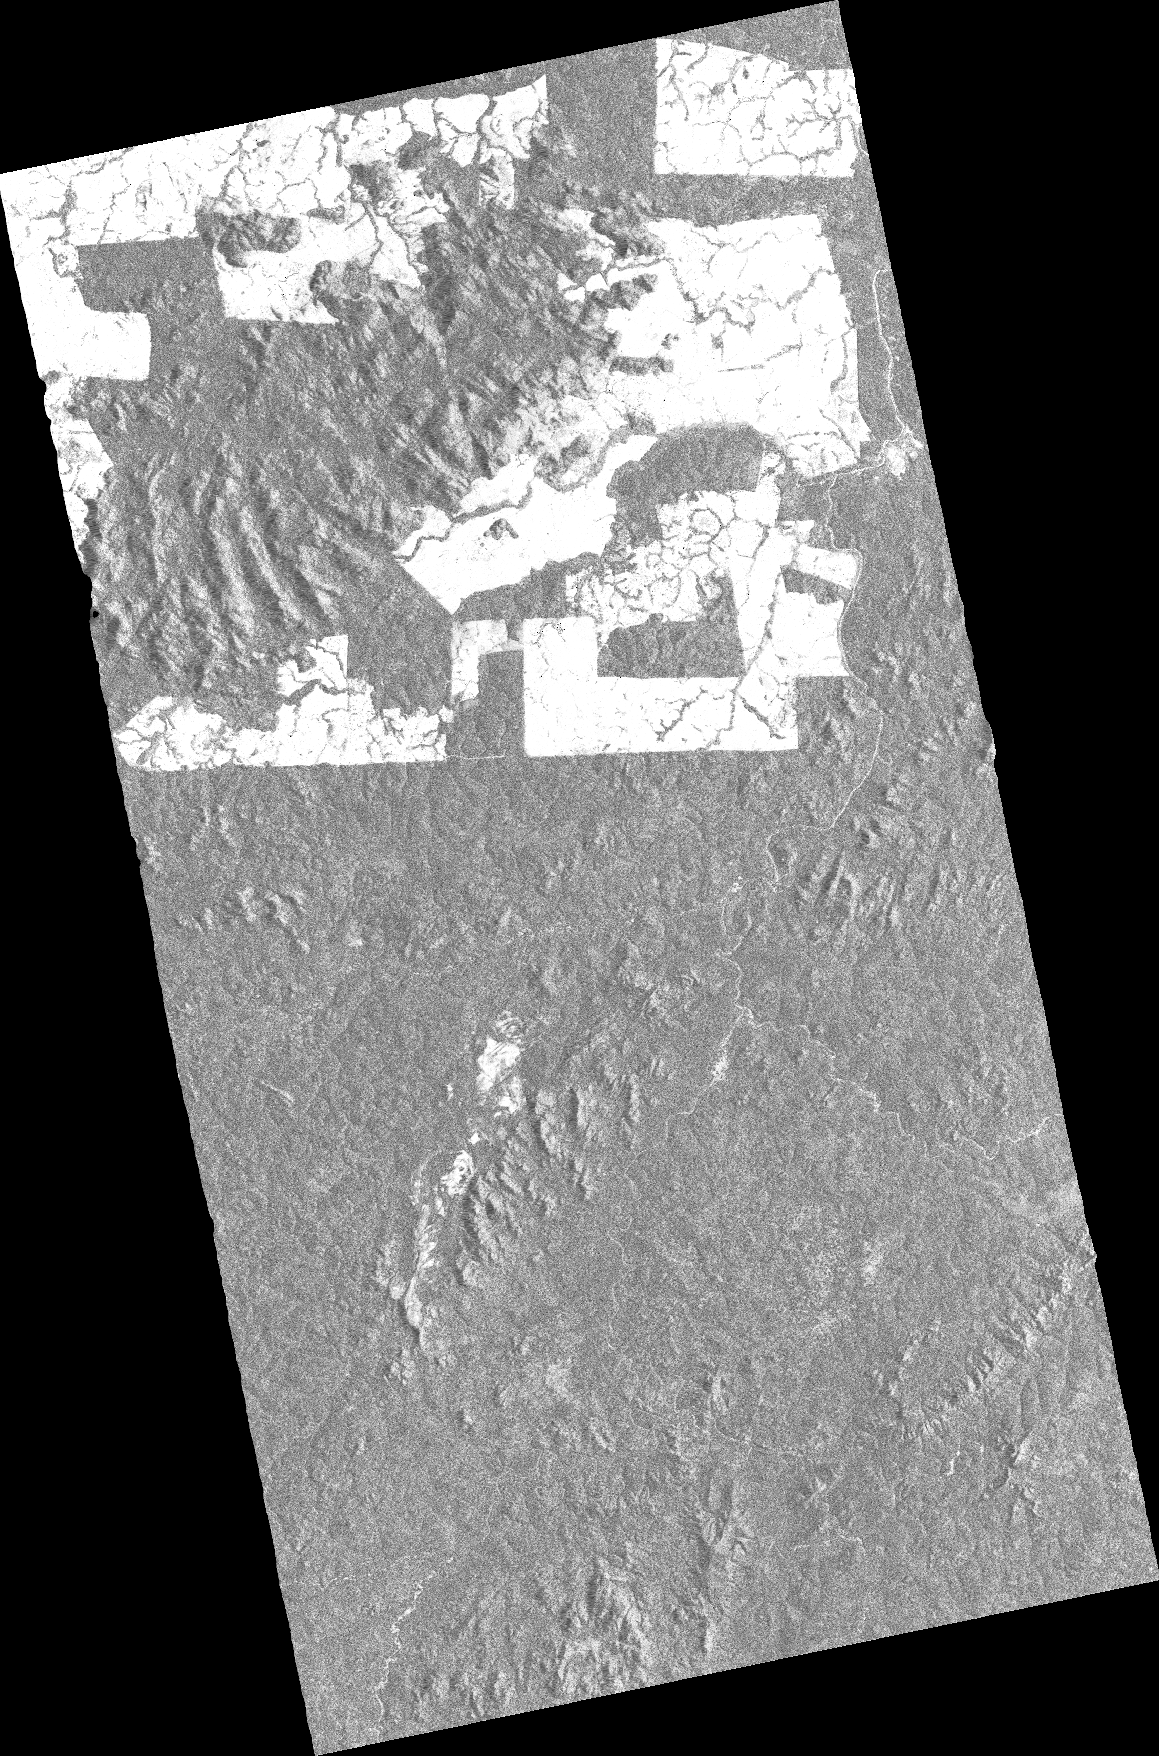
\includegraphics[width=0.8\linewidth]{Chapter4/coSSC_master_gamma_vol.png}
      \caption{Coherence Image of Amazon area.}
    \end{subfigure}
  \caption{Figura}
  \label{fig:asdf}
\end{figure}

Given these two images it will be calculated the result of (\ref{eq:test}) for different displacement vectors
$d=(d_1, d_2)$. It is chosen that the displacement vectors have possibles angle $\theta$ equals to 0$^{\circ}$, 45$^{\circ}$, 90$^{\circ}$ and 135$^{\circ}$, and magnitudes of 1, 2, 3, 4, 5, 6 pixels.
The following tables show the result of the test for the images for areas of forest and deforested areas.



\begin{table}[H]
    \begin{tabular}{ |p{2.5cm}||p{2.5cm}|p{2.5cm}|p{2.5cm}|p{2.5cm}| }
     \hline
     \multicolumn{5}{|c|}{Average Coherence} \\
     \hline
     Distance& $\theta=0$ & $\theta=45$ & $\theta=90$ & $\theta=135$\\
     \hline
        1 &13.46 &7.95 &13.56 &7.96\\
        2 &5.13 &4.06 &5.21 &4.13\\
        3 &4.04 &4.40 &4.13 &4.38\\
        4 &4.19 &5.30 &4.80 &5.18\\
        5 &5.42 &6.71 &5.50 &6.50\\
        6 &6.22 &7.22 &6.39 &6.99\\
     \hline
    
    \end{tabular}
     \caption{$\chi^2$ result for coherence image}
    \label{table:1}
\end{table}

\begin{table}[H]
    \begin{tabular}{ |p{2.5cm}||p{2.5cm}|p{2.5cm}|p{2.5cm}|p{2.5cm}| }
     \hline
     \multicolumn{5}{|c|}{Coherence of forest area} \\
     \hline
     Distance& $\theta=0$ & $\theta=45$ & $\theta=90$ & $\theta=135$\\
     \hline
        1 &13.01 &7.36 &12.68 &7.10\\
        2 &4.52 &3.75 &4.48 &3.77\\
        3 &3.65 &4.32 &3.91 &4.34\\
        4 &4.14 &5.20 &4.58 &5.10\\
        5 &5.12 &6.57 &5.21 &6.41\\
        6 &6.91 &7.06 &6.08 &6.87\\
     \hline
    \end{tabular}
     \caption{$\chi^2$ result for coherence in forest areas}
    \label{table:2}
\end{table}

\begin{table}[H]
    \begin{tabular}{ |p{2.5cm}||p{2.5cm}|p{2.5cm}|p{2.5cm}|p{2.5cm}| }
     \hline
     \multicolumn{5}{|c|}{Coherence of deforested area} \\
     \hline
     Distance& $\theta=0$ & $\theta=45$ & $\theta=90$ & $\theta=135$\\
     \hline
        1 &10.58 &7.28 &10.84 &7.16\\
        2 &4.94 &3.33 &5.37 &3.24\\
        3 &3.26 &2.71 &3.78 &2.63\\
        4 &3.11 &3.20 &3.64 &3.11\\
        5 &3.73 &4.04 &4.09 &3.95\\
        6 &4.29 &4.33 &4.51 &4.29\\
     \hline
    \end{tabular}
     \caption{$\chi^2$ result for coherence in deforested areas}
    \label{table:3}
\end{table}

\begin{table}[H]
    \begin{tabular}{ |p{2.5cm}||p{2.5cm}|p{2.5cm}|p{2.5cm}|p{2.5cm}| }
     \hline
     \multicolumn{5}{|c|}{$\beta^0$ of forest area} \\
     \hline
     Distance& $\theta=0$ & $\theta=45$ & $\theta=90$ & $\theta=135$\\
     \hline
        1 &1.26 &0.63 &1.59 &0.73\\
        2 &0.28 &0.20 &0.42 &0.24\\
        3 &0.22 &0.24 &0.26 &0.23\\
        4 &0.29 &0.29 &0.28 &0.27\\
        5 &0.35 &0.39 &0.31 &0.35\\
        6 &0.39 &0.44 &0.37 &0.39\\
     \hline
    \end{tabular}
     \caption{$\chi^2$ result for $\beta^0$ in forest areas}
    \label{table:4}
\end{table}

\begin{table}[H]
    \begin{tabular}{ |p{2.5cm}||p{2.5cm}|p{2.5cm}|p{2.5cm}|p{2.5cm}| }
     \hline
     \multicolumn{5}{|c|}{$\beta^0$ of deforested area} \\
     \hline
     Distance& $\theta=0$ & $\theta=45$ & $\theta=90$ & $\theta=135$\\
     \hline
        1 &0.82 &0.43 &1.07 &0.50\\
        2 &0.22 &0.14 &0.33 &0.15\\
        3 &0.15 &0.14 &0.20 &0.13\\
        4 &0.17 &0.17 &0.19 &0.16\\
        5 &0.20 &0.22 &0.02 &0.21\\
        6 &0.23 &0.26 &0.23 &0.25\\
     \hline
    \end{tabular}
     \caption{$\chi^2$ result for $\beta^0$ in deforested areas}
    \label{table:5}
\end{table}

Analyzing the tables above we can see that choosing pixels that are closer in the image gives the maximum information for texture calculations (this means that there are no hidden patterns/structures in the images analyzed). According to the tables, until the rest of this work the displacement vector used will always be equals to $d=(0, 1)$.


\subsection{The GLCM textures results}
Let us visualize the texture results for the Coherence image above.
It was computed 7 different textures for the coherence image above: the ASM, contrast, correlation, dissimilarity, energy, entropy and homogeneity.
These textures can be visualized below
\newpage
\begin{figure}[H]
  \centering
  \begin{subfigure}[b]{0.4\linewidth}
    \includegraphics[width=\linewidth]{Chapter4/glcm_textures/ASMimage.png}
     \caption{ASM texture of Coherence Image}
  \end{subfigure}
  \begin{subfigure}[b]{0.4\linewidth}
    \includegraphics[width=\linewidth]{Chapter4/glcm_textures/contrastimage.png}
    \caption{Contrast texture of Coherence Image}
  \end{subfigure}
  \begin{subfigure}[b]{0.4\linewidth}
    \includegraphics[width=\linewidth]{Chapter4/glcm_textures/correlationimage.png}
    \caption{Correlation texture of Coherence Image}
  \end{subfigure}
  \begin{subfigure}[b]{0.4\linewidth}
    \includegraphics[width=\linewidth]{Chapter4/glcm_textures/dissimilarityimage.png}
    \caption{Dissimilarity texture of Coherence Image}
  \end{subfigure}
\end{figure}
\newpage
\begin{figure}[H]\ContinuedFloat
  \begin{subfigure}[b]{0.4\linewidth}
    \includegraphics[width=\linewidth]{Chapter4/glcm_textures/energyimage.png}
    \caption{Energy texture of Coherence Image}
  \end{subfigure}
  \begin{subfigure}[b]{0.4\linewidth}
    \includegraphics[width=\linewidth]{Chapter4/glcm_textures/entropyimage.png}
    \caption{Entropy texture of Coherence Image}
  \end{subfigure}
  \begin{subfigure}[b]{0.4\linewidth}
    \includegraphics[width=\linewidth]{Chapter4/glcm_textures/homogeneityimage.png}
    \caption{Homogeneity texture of Coherence Image}
  \end{subfigure}
\end{figure}

Just by looking at the images above it might be hard to know if they are better suited for classification or not. One solution in order to be able to know quantitatively if they are better to classification is to look at the histogram of the pixels intensity and to compare it with the histograms of the pixels intensity for forest and non forest area in the original coherence image.
For this area it was provided the reference map for comparison, so it is know if a pixel is in a forest area or in a deforested area, and by using this reference map it is possible to make the histograms of the pixel intensity for each area and to compare it with the original histograms for the coherence.
\begin{figure}[H]
  \centering
  \begin{subfigure}[b]{0.4\linewidth}
    \includegraphics[width=\linewidth]{Chapter4/referencemap.png}
     
  \end{subfigure}
  \caption{Reference Map provided by DLR.}
  \label{fig:reference_map}
\end{figure}
From the reference map above it was possible to extract the following probability density function from the histogram of the coherence.
\begin{figure}[H]
  \centering
  \begin{subfigure}[b]{\linewidth}
    \includegraphics[width=\linewidth]{Chapter4/histogramcoherence.png}
     \caption{Probability density Function for Coherence.}
  \end{subfigure}
\end{figure}
It is possible to see that the probability density functions (PDF) overlap at some point, which implies that there is always a probability of error when trying to classify the information of the pixel. On the image above it was also calculated which percentage of the area of one PDF is below the other PDF. For example, from the image above, 3 percent of the forest coherence PDF was below the Non Forest coherence PDF while 16 percent of the non forest coherence PDF was below the forest coherence PDF.
We can see the PDFs obtained from the histograms of the texture features and see whether the PDFs are more separated compared to the PDFs of the coherence.

\begin{figure}[H]
  \centering
  \begin{subfigure}[b]{0.4\linewidth}
    \includegraphics[width=\linewidth]{Chapter4/glcm_textures/ASM_hist.png}
     \caption{Probability density Function for Angular Second Moment.}
  \end{subfigure}
  \centering
  \begin{subfigure}[b]{0.4\linewidth}
    \includegraphics[width=\linewidth]{Chapter4/glcm_textures/contrast_hist.png}
     \caption{Probability density Function for Contrast.}
  \end{subfigure}
  \centering
  \begin{subfigure}[b]{0.4\linewidth}
    \includegraphics[width=\linewidth]{Chapter4/glcm_textures/correlation_hist.png}
     \caption{Probability density Function for Correlation.}
  \end{subfigure}
  \centering
  \begin{subfigure}[b]{0.4\linewidth}
    \includegraphics[width=\linewidth]{Chapter4/glcm_textures/dissimilarity_hist.png}
     \caption{Probability density Function for Dissimilarity.}
  \end{subfigure}
  \centering
  \begin{subfigure}[b]{0.4\linewidth}
    \includegraphics[width=\linewidth]{Chapter4/glcm_textures/energy_hist.png}
     \caption{Probability density Function for Energy.}
  \end{subfigure}
  \centering
  \begin{subfigure}[b]{0.4\linewidth}
    \includegraphics[width=\linewidth]{Chapter4/glcm_textures/entropy_hist.png}
     \caption{Probability density Function for Entropy.}
  \end{subfigure}
  \centering
  \begin{subfigure}[b]{0.4\linewidth}
    \includegraphics[width=\linewidth]{Chapter4/glcm_textures/homogeneity_hist.png}
     \caption{Probability density Function for Homogeneity.}
  \end{subfigure}
\end{figure}

From the images above it is possible to see clearly that the PDFs of the textures are very different from the PDFs of the coherence, that means that the information contained in the textures is different from the information contained in the coherence, which implies that it is information that can be useful for image segmentation and classification, even if the intersection of PDFs is higher than in the coherence's PDF. 


\section{The Laws Textures results}
\label{sec:laws_textures_results}
As mentioned in the previous chapter, the Laws textures are obtained by applying a series of linear filters to the image. Below there are images of the 9 possible texture results of these filters.

\begin{figure}[H]
  \centering
  \begin{subfigure}[b]{0.4\linewidth}
    \includegraphics[width=\linewidth]{Chapter4/laws_textures/e5e5_e5e5image.png}
     \caption{Image of e5e5/e5e5 texture.}
  \end{subfigure}
  \centering
  \begin{subfigure}[b]{0.4\linewidth}
    \includegraphics[width=\linewidth]{Chapter4/laws_textures/e5r5_r5e5image.png}
     \caption{Image of e5r5/r5e5 texture.}
  \end{subfigure}
  \centering
  \begin{subfigure}[b]{0.4\linewidth}
    \includegraphics[width=\linewidth]{Chapter4/laws_textures/e5s5_s5e5image.png}
     \caption{Image of e5s5/s5e5 texture.}
  \end{subfigure}
  \centering
  \begin{subfigure}[b]{0.4\linewidth}
    \includegraphics[width=\linewidth]{Chapter4/laws_textures/l5e5_e5l5image.png}
     \caption{Image of l5e5/e5l5 texture.}
  \end{subfigure}
\end{figure}
\newpage
\begin{figure}[H]\ContinuedFloat
  \centering
  \begin{subfigure}[b]{0.4\linewidth}
    \includegraphics[width=\linewidth]{Chapter4/laws_textures/l5r5_r5l5image.png}
     \caption{Image of l5r5/r5l5 texture.}
  \end{subfigure}
  \centering
  \begin{subfigure}[b]{0.4\linewidth}
    \includegraphics[width=\linewidth]{Chapter4/laws_textures/l5s5_s5l5image.png}
     \caption{Image of l5s5/s5l5 texture.}
  \end{subfigure}
  \centering
  \begin{subfigure}[b]{0.4\linewidth}
    \includegraphics[width=\linewidth]{Chapter4/laws_textures/r5r5_r5r5image.png}
     \caption{Image of r5r5/r5r5 texture.}
  \end{subfigure}
  \centering
  \begin{subfigure}[b]{0.4\linewidth}
    \includegraphics[width=\linewidth]{Chapter4/laws_textures/s5r5_r5s5image.png}
     \caption{Image of s5r5/r5s5 texture.}
  \end{subfigure}
\end{figure}
\newpage
\begin{figure}[H]\ContinuedFloat
  \centering
  \begin{subfigure}[b]{0.4\linewidth}
    \includegraphics[width=\linewidth]{Chapter4/laws_textures/s5s5_s5s5image.png}
     \caption{Image of s5s5/s5s5 texture.}
  \end{subfigure}
\end{figure}
Again we must look at the PDFs for different classes and see whether they are different from the PDF of the coherence.

\begin{figure}[H]
  \centering
  \begin{subfigure}[b]{0.4\linewidth}
    \includegraphics[width=\linewidth]{Chapter4/laws_textures/e5e5_e5e5.png}
     \caption{Probability density Function for e5e5/e5e5.}
  \end{subfigure}
  \centering
  \begin{subfigure}[b]{0.4\linewidth}
    \includegraphics[width=\linewidth]{Chapter4/laws_textures/e5r5_r5e5.png}
     \caption{Probability density Function for e5r5/r5e5.}
  \end{subfigure}
  \centering
  \begin{subfigure}[b]{0.4\linewidth}
    \includegraphics[width=\linewidth]{Chapter4/laws_textures/e5s5_s5e5.png}
     \caption{Probability density Function for e5s5/s5e5.}
  \end{subfigure}
  \centering
  \begin{subfigure}[b]{0.4\linewidth}
    \includegraphics[width=\linewidth]{Chapter4/laws_textures/l5e5_e5l5.png}
     \caption{Probability density Function for l5e5/e5l5.}
  \end{subfigure}
  \centering
  \begin{subfigure}[b]{0.4\linewidth}
    \includegraphics[width=\linewidth]{Chapter4/laws_textures/l5r5_r5l5.png}
     \caption{Probability density Function for l5r5/r5l5.}
  \end{subfigure}
  \centering
  \begin{subfigure}[b]{0.4\linewidth}
    \includegraphics[width=\linewidth]{Chapter4/laws_textures/l5s5_s5l5.png}
     \caption{Probability density Function for l5s5/s5l5.}
  \end{subfigure}
  \centering
  \begin{subfigure}[b]{0.4\linewidth}
    \includegraphics[width=\linewidth]{Chapter4/laws_textures/r5r5_r5r5.png}
     \caption{Probability density Function for r5r5/r5r5.}
  \end{subfigure}
  \centering
  \begin{subfigure}[b]{0.4\linewidth}
    \includegraphics[width=\linewidth]{Chapter4/laws_textures/s5r5_r5s5.png}
     \caption{Probability density Function for s5r5/r5s5.}
  \end{subfigure}
\end{figure}

\newpage
\begin{figure}[H]
  \centering
  \begin{subfigure}[b]{0.4\linewidth}
    \includegraphics[width=\linewidth]{Chapter4/laws_textures/s5s5_s5s5.png}
     \caption{Probability density Function for s5s5/s5s5 texture.}
  \end{subfigure}
\end{figure}




From the images above we can see clearly that the PDFs are more separated than the coherence PDF. A important thing that must be noticed is that all the different textures have very similar PDFs, which might me an indicator that the images are very similar between themselves, and that using more than one texture for classification means adding redundant information for the classification algorithms, which might degrade performance instead of increasing it.

\section{Sum And Difference Histograms Textures}
\label{sec:sum_and_diff_hist_textures}
The last method analyzed for generating textures is the Sum and Difference Histogram Texture. Below there are the texture results for this method.

\begin{figure}[H]
  \centering
  \begin{subfigure}[b]{0.4\linewidth}
    \includegraphics[width=\linewidth]{Chapter4/sum_and_diff_textures/cluster_prominenceimage.png}
     \caption{Cluster Prominence Texture Image}
  \end{subfigure}
  \centering
  \begin{subfigure}[b]{0.4\linewidth}
    \includegraphics[width=\linewidth]{Chapter4/sum_and_diff_textures/cluster_shadeimage.png}
     \caption{Cluster Shade Texture Image}
  \end{subfigure}
  \centering
  \begin{subfigure}[b]{0.4\linewidth}
    \includegraphics[width=\linewidth]{Chapter4/sum_and_diff_textures/contrastimage.png}
     \caption{Contrast Texture Image}
  \end{subfigure}
  \centering
  \begin{subfigure}[b]{0.4\linewidth}
    \includegraphics[width=\linewidth]{Chapter4/sum_and_diff_textures/correlationimage.png}
     \caption{Correlation Texture Image}
  \end{subfigure}
\end{figure}
\newpage
\begin{figure}[H]\ContinuedFloat
  \centering
  \begin{subfigure}[b]{0.4\linewidth}
    \includegraphics[width=\linewidth]{Chapter4/sum_and_diff_textures/energyimage.png}
     \caption{Energy.}
  \end{subfigure}
  \centering
  \begin{subfigure}[b]{0.4\linewidth}
    \includegraphics[width=\linewidth]{Chapter4/sum_and_diff_textures/entropyimage.png}
     \caption{Entropy Texture Image}
  \end{subfigure}
  \centering
  \begin{subfigure}[b]{0.4\linewidth}
    \includegraphics[width=\linewidth]{Chapter4/sum_and_diff_textures/homogeneityimage.png}
     \caption{ Homogeneity Texture Image}
  \end{subfigure}
  \centering
  \begin{subfigure}[b]{0.4\linewidth}
    \includegraphics[width=\linewidth]{Chapter4/sum_and_diff_textures/meanimage.png}
     \caption{Mean Texture Image}
  \end{subfigure}
\end{figure}
\newpage
\begin{figure}[H]\ContinuedFloat
  \centering
  \begin{subfigure}[b]{0.4\linewidth}
    \includegraphics[width=\linewidth]{Chapter4/sum_and_diff_textures/varianceimage.png}
     \caption{Variance Texture Image}
  \end{subfigure}
\end{figure}
Again we must analyze the histograms to see if these features really are useful for classification and segmentation of a image.

\begin{figure}[H]
  \centering
  \begin{subfigure}[b]{0.4\linewidth}
    \includegraphics[width=\linewidth]{Chapter4/sum_and_diff_textures/cluster_prominence_hist.png}
     \caption{Probability density Function for Cluster Prominence.}
  \end{subfigure}
  \centering
  \begin{subfigure}[b]{0.4\linewidth}
    \includegraphics[width=\linewidth]{Chapter4/sum_and_diff_textures/cluster_shade_hist.png}
     \caption{Probability density Function for Cluster Shade.}
  \end{subfigure}
  \centering
  \begin{subfigure}[b]{0.4\linewidth}
    \includegraphics[width=\linewidth]{Chapter4/sum_and_diff_textures/contrast_hist.png}
     \caption{Probability density Function for Contrast.}
  \end{subfigure}
  \centering
  \begin{subfigure}[b]{0.4\linewidth}
    \includegraphics[width=\linewidth]{Chapter4/sum_and_diff_textures/correlation_hist.png}
     \caption{Probability density Function for Correlation.}
  \end{subfigure}
  \centering
  \begin{subfigure}[b]{0.4\linewidth}
    \includegraphics[width=\linewidth]{Chapter4/sum_and_diff_textures/energy_hist.png}
     \caption{Probability density Function for Energy.}
  \end{subfigure}
  \centering
  \begin{subfigure}[b]{0.4\linewidth}
    \includegraphics[width=\linewidth]{Chapter4/sum_and_diff_textures/entropy_hist.png}
     \caption{Probability density Function for Entropy.}
  \end{subfigure}
\end{figure}

\begin{figure}[H]\ContinuedFloat

  \centering
  \begin{subfigure}[b]{0.4\linewidth}
    \includegraphics[width=\linewidth]{Chapter4/sum_and_diff_textures/homogeneity_hist.png}
     \caption{Probability density Function for Homogeneity.}
  \end{subfigure}
  
  \centering
  \begin{subfigure}[b]{0.4\linewidth}
    \includegraphics[width=\linewidth]{Chapter4/sum_and_diff_textures/mean_hist.png}
     \caption{Probability density Function for Mean.}
  \end{subfigure}
  
  \centering
  \begin{subfigure}[b]{0.4\linewidth}
    \includegraphics[width=\linewidth]{Chapter4/sum_and_diff_textures/variance_hist.png}
     \caption{Probability density Function for Variance.}
  \end{subfigure}
  
\end{figure}

From the histograms and the texture images it is clear that some of the textures are excellently suited for classification, specially the Cluster Shade and Cluster Prominence textures which provide excellent separation between the probability density function. From those images it is clear that in the case of the TANDEM-X the sum and difference histogram methods for texture provided a significantly better result than the other textures, so through the rest of the work there will be a focus in using this method instead of the others, since due to computational limitations is not viable to use all texture methods for classification, since it takes a very long time to compute them.
